\documentclass[10pt]{article}
\usepackage{graphicx}

\everymath{\displaystyle}

\begin{document}
  \title{Specification for Ultrasound Transmitter and Receiver Pair}
  \author{Sam Mansfield, Edward Lee, and Ben Zhang\\
          Fall 2013}
  \maketitle

  \section{Overview}
    The basic idea of this project is to create a small device that can be plugged into an outlet, that transmits a unique ultrasonic bit pattern (controlled by switches). This transmitter would have a receiver pair part of an app on a smartphone that can decipher the ultrasonic bit pattern. From the deciphered signal the app would be able to distinguish what room it is located in. So ideally, an transmitter would be placed in each room and the receiver would roam from room to room.
  
  \section{Concept}
    \subsection{Matched Filters}
      The idea of a matched filter is that the transmitter will send out a specific signal, which is either present of not present. The receiver will have a matched filter signal, that will be convolved with the incoming signal that produces a filtered signal that can then be analyzed. Based on Digital Communication 2nd Ed by Edward Lee and David Messerschmitt, the following are good signals to use, where h(t) represents the transmitted signal and f(t) represents the matched filter:
        \[h(t) = f(t) = \frac{4\alpha}{\pi T}\frac{cos((1 + \alpha)\pi t/T) + Tsin((1-\alpha)\pi t/T)/(4\alpha t)}{1 - (4\alpha t/T)^2}\]
        \[H(j\omega) = F(j\omega) = \sqrt{P(j\omega)}\]
        \[p(t) = \frac{sin(\pi t/T)}{\pi t/T}\frac{cos(\alpha \pi t/T}{1 - (2\alpha t/T)^2}\]
      By convolving h(t) and f(t), p(t) will be extracted and can then be sampled and this reduces the noise that gets mixed in with the transmitted signal. T in these equations is the Baud Rate and \(\alpha\) is how quickly the signal will roll off after T, 0 being the least roll off and 1 being the biggest roll off (having an \(\alpha\) greater than 1 is not recommended in this case because of excess bandwidth).

    \subsection{Serial Transfer}
      To communicate several bits of data a serial protocol of sorts will be used. A start bit followed by 8 bits followed by a stop bit will be sent each signal.\\[1em]
        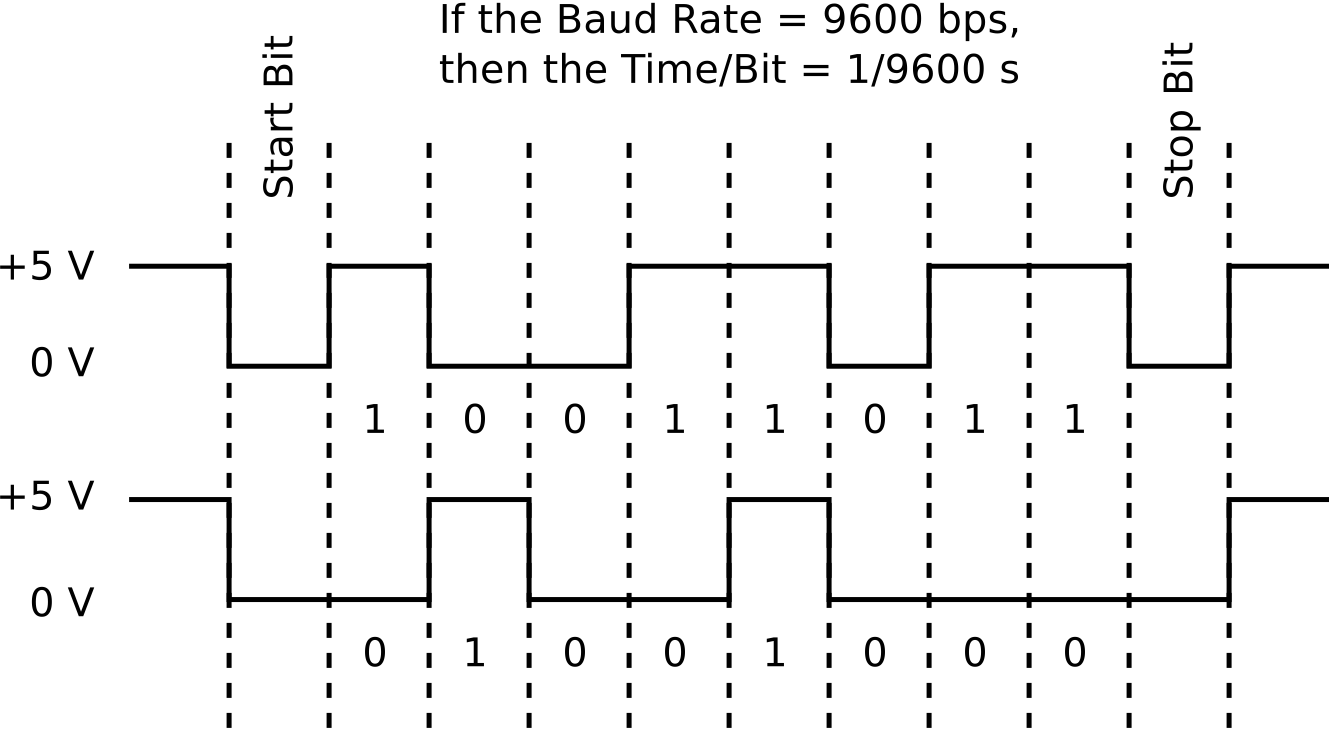
\includegraphics[scale=0.5]{./diagrams/SerialCommunication}\footnote{taken from http://www.fiz-ix.com/2013/02/introduction-to-arduino-serial-communication/}
      
  \section{Building Blocks}
    \subsection{Ptolemy}
      The first steps are to create a transmitter and receiver on a computer (probably using ptolemy) for proof of concept. Begin able to implement the matched filter design will make it so that it can be used to test the hardware.
      \subsubsection{Questions with Ptolemy}
        \begin{enumerate}
          \item How do I set the frequency that I am sending raised cosines. I understand that I am sending a raised cosine (or not a raised cosine) every T intervals. But, how do I set the rate that the samples are being transmitted?
        \end{enumerate}

    \subsection{Building the Hardware}
      The next step is to create the hardware. I will probably use a teensy 3.0. It has a hardware multiply and I'm familiar with it. I also need to find a speaker that can produce sound in the 20-22kHz range. They way I understand it, I need to send analog output to the speaker and update it based on an array of values that a raised cosine takes on.
      \subsubsection{A Look at the Teensy 3, capabilities}
        The Teensy 3's clock speed can be overclocked to 96MHz. In order to play 20kHz, we need at least 40kHz sample rate. 

  \section{Designing an IIR Filter}
    I am designing an IIR filter in Ptolemy that can listen to the hardware emitter and recognize if the signal is present or not present. To do this I need to find the coefficients of the IIR filter (ai and bi), which for Ptolemy are represented by:
      \[H(z) = \frac{\sum_{i=0}^{P} b_i z^{-i}}{\sum_{j=0}^{Q} a_i z^{-j}}\]

    To create a bandpass filter you need two matching poles at the designated \(\theta\) and the following equation will give you the coefficients:
      \[H(z) = \frac{1}{(1 - 0.99e^{i\theta}z^{-1})(1 - 0.99e^{-i\theta}z^{-1})}\]
      \[H(z) = \frac{1}{1 - 0.99(e^{i\theta} + e^{-i\theta})z^{-1} + 0.99^2z^{-2}}\]
      \[H(z) = \frac{1}{1 - 2*0.99(\frac{e^{i\theta} + e^{-i\theta}}{2})z^{-1} + 0.99^2z^{-2}}\]
      \[H(z) = \frac{1}{1 - 2*0.99cos(\theta)z^{-1} + 0.99^2z^{-2}}\]
      
      %Plug into Wolframalpha 
      %1/(1 - 2*0.99*cos(pi*5000/22050)x^1 + 0.99^2*x^2)
    For a \(\theta\) at 21kHz we can use the information that half of the sampling frequency (44.1kHz) will correspond with \(\pi\) so to find the corresponding \(\theta\) can be determined from the following formula: \(\theta = \frac{21,000}{22.050}*\pi\).
\end{document}
